\renewcommand{\thesection}{A}
%************************************************
\chapter{Special functions}\label{sec: functions}
%************************************************
A collection of useful (non-in-built) functions.
\bigskip

\begin{itemize}
\item[-] \emph{Mode}:
\begin{verbatim}
mode <- function(x) {
	ux <- unique(x)
	ux[which.max(tabulate(match(x, ux)))]
}
	
R: mode(quarks$flavour)
[1] "strange"
\end{verbatim}
	
\item[-]\emph{na2zero}:
\begin{verbatim}
na2zero <- function(x) {
	x[] <- lapply(x,function(x){x[is.na(x)] <- 0; x})
	x
}
\end{verbatim}
	
\item[-]\emph{Cartesian product}
\begin{verbatim}
cross.join <- function(a, b) {
	idx <- expand.grid(seq(length=nrow(a)), 
                           seq(length=nrow(b)))
	cbind(a[idx[,1],], b[idx[,2],])
}
\end{verbatim}
	
 \item[-]\emph{Shapiro $p$-value rejections}
\begin{verbatim}
shapiro.p.value <- function(my.column) {
	my.p.value <- '0.05'
	if(shapiro.test(my.column)[2] < my.p.value){
		return("rejected")
	} else {
		return("not rejected")
	}
}
	
R: iris[, lapply(.SD, shapiro.p.value), by = Species]
      Species Sepal.Length  Sepal.Width Petal.Length   
1:     setosa not rejected not rejected not rejected 
2: versicolor not rejected not rejected not rejected 
3:  virginica not rejected not rejected not rejected 
\end{verbatim}
 \item[-] \emph{Anagrams}
\begin{verbatim}
sort.word <- function(x){
 x <- tolower(x)
 x <- str_replace_all(x, fixed(" "), "")    
 x <- paste(sort(unlist(strsplit(x, ""))), collapse = "") 
 return(x)
}

is.anagram <- function(x,y){
    return(sort.word(x) == sort.word(y))
}

first  <- "Eleven plus Two"
second <- "Twelve plus One"

R: is.anagram(first, second) 
[1] TRUE
\end{verbatim}

 \item[-] \emph{Outliers by clustering}
\begin{verbatim}
outlier.by.clustering <- function(df,N,M){
    cluster   <- kmeans(df, centers = N)
    centres   <- cluster$centers[cluster$cluster,]
    distances <- sqrt(rowSums((df-centres)^2))
    outliers  <- head(df[order(distances, 
                      decreasing = TRUE),],M)
    return(outliers)
}

R: outlier.by.clustering(mtcars[,1:7], 5, 5)

                     mpg cyl disp  hp drat    wt  qsec
Maserati Bora       15.0   8  301 335 3.54 3.570 14.60
Cadillac Fleetwood  10.4   8  472 205 2.93 5.250 17.98
Lincoln Continental 10.4   8  460 215 3.00 5.424 17.82
Hornet Sportabout   18.7   8  360 175 3.15 3.440 17.02
Pontiac Firebird    19.2   8  400 175 3.08 3.845 17.05
\end{verbatim}

\end{itemize}

\begin{comment}
\section{RXKCD}
\texttt{install.packages(RXKCD)}\\
\texttt{library(RXKCD)}
\bigskip

The above fetches comic strips from 
\verb+XKCD+\footnote{
\url{http://xkcd.com/}
}

\texttt{R: getXKCD(which = "random")}
\begin{figure}[!h]
 \centering 
 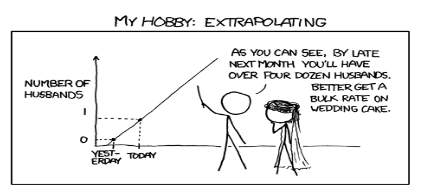
\includegraphics[scale=0.7]{images/xkcd}
 \caption{XKCD strip fetched in \texttt{R}} 
\end{figure}


\section{Colour palette}
I have used the following colour palette
(inspired from ``Solarized''%
\footnote{
\url{http://ethanschoonover.com/solarized}
})
\begin{itemize}
 \item[-] Background: \#002b36
 \item[-] Bars:       \#657b83
 \item[-] Lines:      \#2aa198, \#268bd2
\end{itemize}
\end{comment}



